% !TEX program = xelatex
\documentclass[UTF8,a4paper,zihao=-4,fontset=fandol]{ctexart}
\usepackage[margin=2.3cm]{geometry}
\usepackage{amsmath,amssymb,booktabs,longtable,graphicx,float,tabularx}
\usepackage{xcolor,tikz,fancyhdr,hyperref,caption}
\usepackage{xurl,placeins,needspace,listings}
\usetikzlibrary{arrows.meta,positioning}
\hypersetup{colorlinks=true,linkcolor=black,urlcolor=blue,citecolor=black,pdftitle={考虑预测误差与合同调整成本的微网储能及购电调控策略}}
\definecolor{navy}{HTML}{235789}
\graphicspath{{../figures/}{../../deliverables/candidate_figures/v3_3d/}{../../deliverables/candidate_figures/v2/}{../../deliverables/candidate_figures/v1/}}
\captionsetup{font=small,labelfont=bf,labelsep=quad,skip=7pt,width=.94\linewidth}
\setlength{\headheight}{16pt}
\pagestyle{plain}
\setlength{\parindent}{2em}\setlength{\parskip}{0.12em}
\linespread{1.08}
\setlength{\textfloatsep}{12pt plus 2pt minus 2pt}
\setlength{\intextsep}{12pt plus 2pt minus 2pt}
\renewcommand{\topfraction}{.92}\renewcommand{\bottomfraction}{.85}
\renewcommand{\textfraction}{.06}\renewcommand{\floatpagefraction}{.7}
\ctexset{section={format=\Large\sffamily\bfseries,beforeskip=16pt,afterskip=9pt},subsection={format=\large\sffamily\bfseries,beforeskip=11pt,afterskip=6pt}}
\raggedbottom
\setlength{\emergencystretch}{1em}
\newcommand{\fig}[3]{\begin{figure}[H]\centering\includegraphics[width=#2\linewidth]{#1.pdf}\caption{#3}\end{figure}}
\renewcommand{\arraystretch}{1.1}
\lstset{language=Python,basicstyle=\ttfamily\fontsize{8}{9.5}\selectfont\linespread{1}\selectfont,
  keywordstyle=\bfseries\color{navy},commentstyle=\color{black!55},stringstyle=\color{black!70},
  numbers=left,numberstyle=\tiny\color{black!45},numbersep=7pt,firstnumber=1,
  frame=tb,rulecolor=\color{black!30},framerule=.35pt,
  breaklines=true,breakatwhitespace=false,columns=fullflexible,keepspaces=true,
  showstringspaces=false,tabsize=4,xleftmargin=1.8em,
  aboveskip=7pt,belowskip=7pt,captionpos=t}
\renewcommand{\lstlistingname}{代码}
\title{\heiti 考虑预测误差与合同调整成本的\\微网储能及购电调控策略}
\author{}\date{}
\begin{document}
\maketitle\vspace{-3em}\thispagestyle{plain}
\begin{abstract}
针对光伏出力、用电负荷与外网电价变化下的微网购电及储能调控问题，建立考虑预测误差与合同调整成本的优化模型。以10分钟为决策时段，统一描述能量平衡、充放电损耗、功率上限及储电量边界，采用线性规划与充放电互斥校验求解调度计划，并按“时段开始决策、时段结束结算”区分可用信息与实际偏差。

针对第一问，建立代表日确定性调度模型，得到全天购电量59482.699 kWh、购电费用35126.95元，相比无储能方案降低26.90\%。针对第二问，利用历史净负荷残差的分时分位数构造安全裕量，在一月选择参数后，对二月至十二月334天进行固定参数回放。所得总费用为15137987.06元，较无裕量基线降低8.71\%；其作用机制是增加较低价格的计划购电，减少按5倍电价结算的应急购电。

针对第三问，将新增预报的价值与合同调整费用共同纳入决策。裕量零点固定策略总费用为15129676.16元，逐次使用新预报重规划反而增费3.66\%。进一步采用预期净收益门控，总费用降至15122320.83元，但相对固定策略仅改善0.0486\%，且月度收益不稳定，因而保留裕量固定策略作为简洁方案。针对第四问，在目标日电价曲线提前可知的假设下，将相同方法用于动态电价：安全裕量降费8.58\%，新预报重规划仍增费3.35\%，两项主要结论与固定电价下相符。

参数响应面和月均储电量曲面分别刻画了安全裕量的局部敏感性与全年日内运行规律。进一步分析表明，当日前计划无富余且储能执行既定动作时，应急电量由修正后的净负荷预测残差决定；电价主要改变计划购电的时段分配。研究说明，预测改进应以实际总费用衡量，增加预报频率或优化频率并不必然带来经济收益。

\end{abstract}
\noindent\textbf{关键词：}微网；储能调度；日前购电；分位数安全裕量；合同调整；因果控制
\newpage
\FloatBarrier
\section{问题分析与研究路线}
微网通过光伏、本地储能与外网购电满足小区负荷。储能将电量在时段间转移，但充放电损耗、容量及功率限制意味着低价多购电并不总能抵消后续高价缺口。题目四问依次增加负荷及光伏不确定性、预报更新与合同调整、动态电价，核心目标始终是满足物理约束后的实际购电总费最小\cite{problem}。

第一问以给定日曲线建立确定性优化；第二问在零点锁定合同后承担预测偏差产生的5倍应急费用；第三问在6、12、18点比较保持合同与更新合同的代价；第四问将固定日价格向量替换为动态价格。本文将预测、合同优化、储能执行和费用结算分开建模。已有研究将混合整数规划与模型预测控制用于微网运行优化\cite{parisio}；本文据题目给定的应急电价与违约费用，重点考察预测信息改善能否转化为实际费用下降。
\begin{figure}[H]\centering
\begin{tikzpicture}[box/.style={draw=navy,rounded corners=2pt,minimum width=2.5cm,minimum height=.85cm,align=center},>=Stealth,node distance=1.35cm]
\node[box](pv){光伏发电};\node[box,right=of pv](bus){微网母线};\node[box,right=of bus](load){小区负载};
\node[box,below=of pv](grid){外部电网};\node[box,below=of bus](battery){储能设备};\node[box,below=of load](w){无收益富余};
\draw[->,thick](pv)--(bus);\draw[->,thick](bus)--(load);\draw[->,thick](grid)--node[above,sloped,font=\small]{计划及应急购电}(bus);\draw[<->,thick](bus)--(battery);\draw[->,thick](bus)--(w);
\end{tikzpicture}
\caption{微网能量流结构。箭头表达连接关系，不代表电量大小；不设售电收入。}
\end{figure}
本文不把最小预测误差直接等同于最低购电成本，而以统一回放中的总费用选择方案。各模型在同一效率、日终储电量和计费解释下比较；改变这些解释得到的费用差应归为假设敏感性。

\FloatBarrier
\section{数据、时间轴与模型假设}
\subsection{数据来源及评价范围}
附件1提供代表日价格、负荷及光伏预测功率；附件2提供2025年全年实际负荷与光伏功率；附件3提供每天四次发布的未来24小时整点光伏预报；附件4提供动态电价；附件5为结果模板\cite{problem}。现有标准化表分别包含144、52560、35040和52560条记录，分别对应代表日、全年实际数据、全年发布预报与全年价格序列。

年度方案的一月用于初始化与开发，二月至十二月为334天固定回放。第二问基线负荷取上周同一时段，光伏取昨日同一时段。安全裕量与门控参数均在一月选择，再冻结至二月起使用。以下结果属于同一年度数据上的回放比较，参数开发与评价时段分开，不将其视为跨年度泛化检验。

\fig{annual_patterns}{1}{全年实际负荷、光伏与净负荷的时间结构。热力图每格对应一天中的一个10分钟物理槽；季节曲线为中位数，阴影为逐槽10\%至90\%经验分位范围，非置信区间。此图用于描述已发生数据，不向决策器提供未来信息。}


\subsection{时间离散与区间对应}\label{sec:time}
一天划分为144个区间，$I_t=[t\Delta,(t+1)\Delta)$，$\Delta=1/6$小时，$t=0,\ldots,143$；储电量定义在145个区间边界上。输入时间标签为00:10至次日00:00。为对应题面00:00至24:00的充放电统计区间与日终储电量约束，本文将标签$T$的采样值用于以$T$结束的时段，采用右端保持近似：
\begin{equation}
L_t=\int_{t\Delta}^{(t+1)\Delta}P^L(s)\,\mathrm ds
\approx P^L((t+1)\Delta)\Delta,\qquad
V_t\approx P^{PV}((t+1)\Delta)\Delta.
\end{equation}
其中功率单位为kW，电量单位为kWh。10:00--10:10时段取10:10的输入采样值，储电量$E_{60}$与$E_{61}$分别表示该时段起止状态。结果模板购电页的印刷标签相对上述物理区间晚10分钟，本文按列位置对应144个时段，正文统一使用物理区间。

当同一日的两个午夜采样均可用时，右端保持与梯形积分的总电量差满足
\begin{equation}\label{eq:gap}
Q_{\mathrm{right}}-Q_{\mathrm{trap}}
=\frac{\Delta}{2}\,[P(24{:}00)-P(0{:}00)].
\end{equation}
相邻日共用午夜端点，因此全年差值可逐日相消至年初、年末两端。在本年度数据中，负荷总电量差为21.77 kWh，光伏差为零；单时段差异仍可能较大。代表日重解中，不同积分规则下优化费用的跨度为0.68\%，储能相对无储能的降费比例为26.66\%至27.24\%。这说明代表日的定性结论对所比较的积分方式较稳定，但总电量差不能直接作为优化费用差的普遍上界。

\subsection{模型假设与主要符号}
储能额定容量12000 kWh，工作能量1200至10800 kWh，最大充放电功率5000 kW。将题面“充放电效率90\%”解释为各方向效率均为0.9；充放电量定义在母线侧。第一问要求日初日末相同，为统一比较，第二至四问也设置每日初末储电量为6000 kWh。这是本文采用的日循环假设；跨日储能调配不在本模型范围内。
\begin{table}[H]\centering\caption{主要变量及单位}
\begin{tabular}{lll}\toprule 符号 & 含义 & 单位\\\midrule
$G_t$ & 当前适用的计划购电量 & kWh\\
$C_t,D_t$ & 母线侧充电量、放电量 & kWh\\
$U_t,W_t$ & 紧急购电量、无收益富余 & kWh\\
$E_t$ & 槽首储电量 & kWh\\
$L_t,V_t$ & 实际负荷电量、光伏电量 & kWh\\
$p_t$ & 普通购电电价 & 元/kWh\\
$\widehat L_t,\widehat V_t$ & 决策时可得预测电量 & kWh\\\bottomrule\end{tabular}
\end{table}
不考虑售电收益和未在题面给出的电池折旧收费。应急购电允许补齐剩余缺口；该模型将外网作为槽末剩余能量结算来源，并未模拟秒级供电过程。

\FloatBarrier
\section{统一优化与严格因果执行}
\subsection{物理约束及确定性求解}
在任一时段，能量平衡及状态转移为
\begin{align}
G_t+V_t+D_t+U_t &= L_t+C_t+W_t,\\
E_{t+1}&=E_t+\eta_c C_t-D_t/\eta_d,\\
1200\le E_t&\le10800,\qquad E_0=E_{144}=6000,\\
0\le C_t,D_t&\le5000\Delta=833.333\ldots,\qquad G_t,U_t,W_t\ge0.
\end{align}
为避免同时充放电，必要时引入$z_t\in\{0,1\}$并约束$C_t\le833.333z_t$、$D_t\le833.333(1-z_t)$。先求线性松弛\cite{boyd}并检查充放互斥；若不满足，则加入整数约束重新求解。通过互斥检查的松弛最优解同时是原问题的可行最优解。

第一问与日前规划以预测电量替换实际电量，令$U_t=0$并最小化$\sum_t p_tG_t$。第二问合同锁定后，实际费用为
\begin{equation}\label{eq:cost}
J_2=\sum_{t=0}^{143}p_tG_t+\sum_{t=0}^{143}5p_tU_t.
\end{equation}
计划购电按承诺付费，富余不退款；紧急购电费用已经含5倍系数。

\subsection{信息集与执行顺序}
定义槽首信息集$\mathcal F_t$包含已发布预测、当前储电量、此前已完成时段的实际数据及可知价格。要求$(C_t,D_t)=\pi_t(\mathcal F_t)$。本槽结束后才获得的$L_t,V_t$不能参与本槽储能动作。动作锁定后结算
\begin{equation}
U_t=[L_t+C_t-G_t-V_t-D_t]_+,\qquad
W_t=[G_t+V_t+D_t-L_t-C_t]_+.
\end{equation}
这保证离散能量平衡，但不等同于已验证瞬时功率控制。当前严格模型中，实际误差由外网与富余项吸收，电池状态按既定动作转移；因此仅观察SOC未必提供额外净负荷信息。
\begin{figure}[H]\centering
\begin{tikzpicture}[>=Stealth,box/.style={draw=navy,align=center,text width=3.45cm,minimum height=1cm},node distance=.6cm]
\node[box](a){槽首 $t$\\读取可用信息，锁定$C_t,D_t$};
\node[box,right=of a](b){执行区间 $I_t$\\本槽真实总量尚未完整获得};
\node[box,right=of b](c){槽末 $t+1$\\观测$L_t,V_t$，结算$U_t,W_t$};
\draw[->,thick](a)--(b);\draw[->,thick](b)--(c);
\end{tikzpicture}
\caption{严格槽首决策、槽末结算时序。当前槽最终实际值不存在指向槽首动作的反向箭头。}
\end{figure}

\subsection{日终可达性及执行器比较}
若状态$E_{t+1}$之后还剩$n$个槽，为保持日终6000可达，约束
\begin{equation}
\max(1200,6000-n\eta_c\bar C)\le E_{t+1}\le
\min(10800,6000+n\bar D/\eta_d).
\end{equation}
基线执行器B0根据可用预测净缺口决定充放电，并施加SOC及上述可达性约束。小时级MPC执行器B1固定日前$G$，每6槽重解余日问题，目标为预测应急费$\sum_{\tau\ge t}5p_\tau\widehat U_\tau$最小，只执行最近6槽。已有计划费是沉没成本，不重复纳入该执行优化。两者的预测在零点冻结，本次MPC没有新增日内预测误差修正。

\FloatBarrier
\section{第一问：代表日调度}
无储能、规则控制与优化控制的日费用分别为48052.05、43949.49和35126.95元。优化方案全天购电59482.699 kWh，相对无储能费用下降26.90\%。图\ref{fig:q1}呈现负荷与光伏、电池充放电及储电量；低价购电、光伏消纳和高价放电须共同满足容量及日终约束，不能只凭峰谷价差逐槽独立决策。
\begin{figure}[H]\centering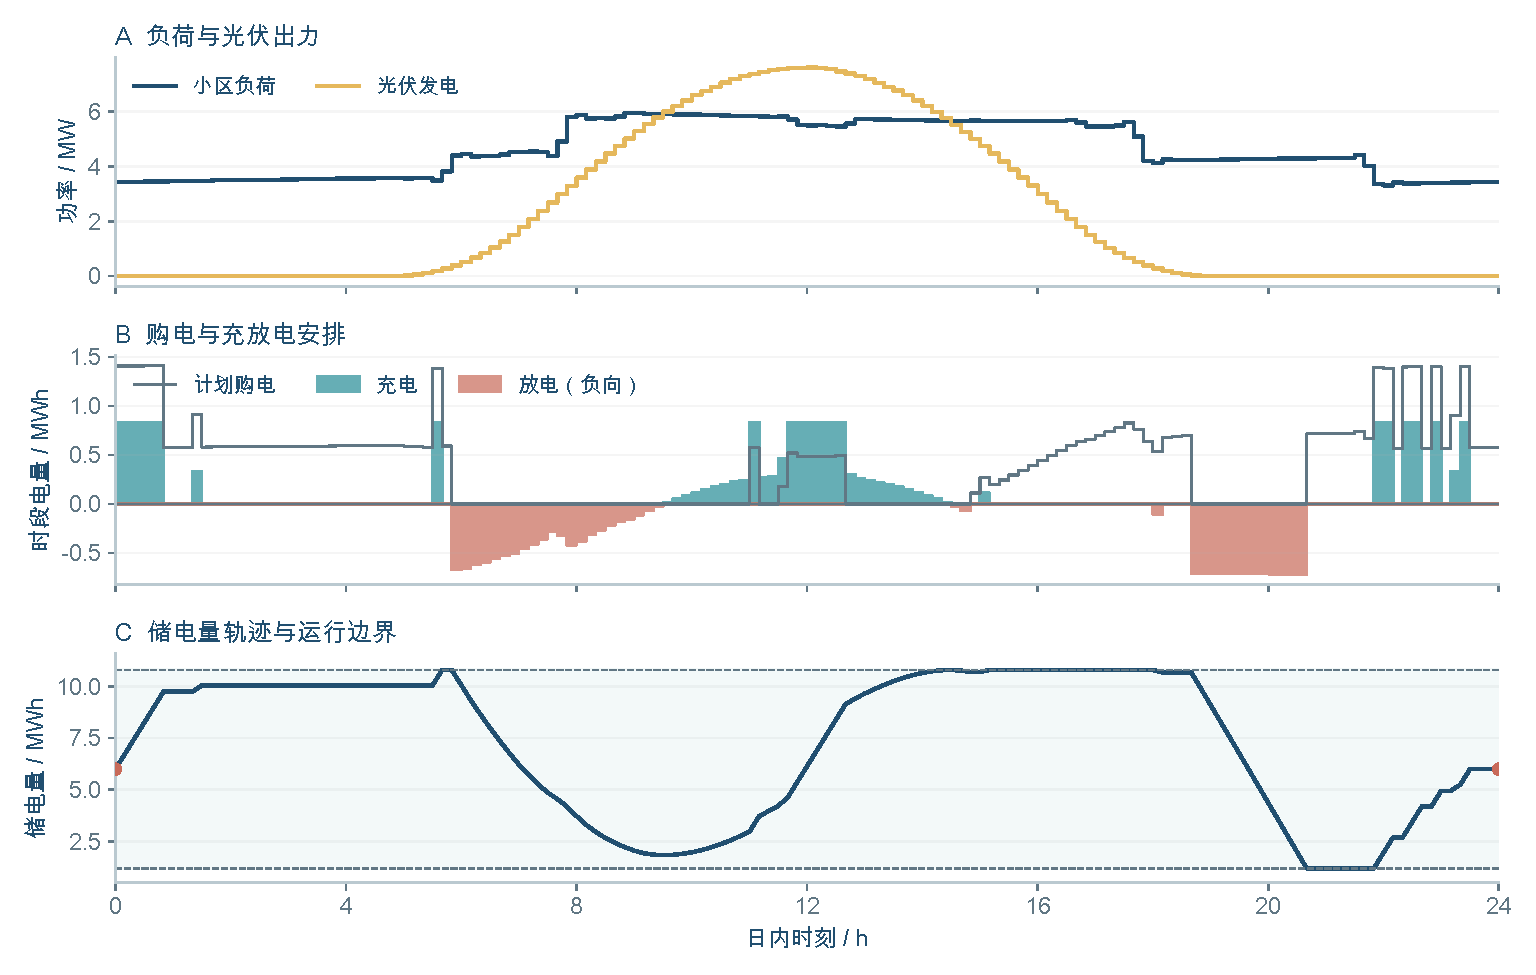
\includegraphics[width=.80\linewidth]{representative_dispatch.pdf}\caption{第一问优化调度。电量曲线按物理槽首绘制，储电量按区间边界绘制；放电以负值表示方向。}\label{fig:q1}\end{figure}
\begin{table}[H]\centering\caption{第一问指定物理时段的购电与充放电}\small
\begin{tabular}{lr}
\toprule
物理时段 & 购电量/kWh \\
\midrule
10:00--10:10 & 0.000 \\
12:00--12:10 & 480.412 \\
14:00--14:10 & 0.000 \\
16:00--16:10 & 445.432 \\
18:00--18:10 & 531.894 \\
20:00--20:10 & 0.000 \\
\bottomrule
\end{tabular}
\quad\begin{tabular}{lrr}
\toprule
物理时段 & 充电量/kWh & 放电量/kWh \\
\midrule
00:00--04:00 & 4500.000 & 0.000 \\
04:00--08:00 & 833.333 & 6365.841 \\
08:00--12:00 & 4787.964 & 1702.997 \\
12:00--16:00 & 5286.035 & 91.101 \\
16:00--20:00 & 0.000 & 5780.132 \\
20:00--24:00 & 5333.333 & 2859.868 \\
\bottomrule
\end{tabular}

\end{table}
日初和日末储电量均为6000 kWh。将90\%改为往返效率并对称分配到两个方向时，已有敏感性结果为33801.50元，比主口径低1325.45元；这是效率假设变化，不是算法节省。

\FloatBarrier
\section{第二问：成本敏感的安全裕量}
\subsection{预测残差与一月选型}
基础预测为$\widehat L_{d,t}=L_{d-7,t}$、$\widehat V_{d,t}=V_{d-1,t}$。历史净负荷残差记为
\begin{equation}
e_{d,t}=(L_{d,t}-V_{d,t})-(\widehat L_{d,t}-\widehat V_{d,t}).
\end{equation}
把一天分为6个四小时桶，在目标日前28日的已完成历史中，计算桶内原始残差分位数$q_{\tau,b}$；历史残差日不足7天时使用零裕量。修正预测为
\begin{equation}
\widetilde L_{d,t}=\widehat L_{d,t}+\kappa\max(0,q_{\tau,b(t)}),\qquad
\widetilde V_{d,t}=\widehat V_{d,t}.
\end{equation}
直接对原始残差求分位数，避免另加偏差项造成重复修正。候选包括零裕量及以下参数形成的八个组合：
\[\tau\in\{0.6,0.7,0.8,0.9\},\qquad\kappa\in\{0.5,1\}.\]
一月8日至14日建立残差历史，一月15日至31日比较完整实际成本，选择$\tau=0.8,\kappa=1$。二月起参数冻结，残差库仍只使用目标日前已经发生的数据。0.8是该候选网格的实测选择，不是由5倍价格在含储能情形下推导出的解析最优值。

\begin{figure}[H]\centering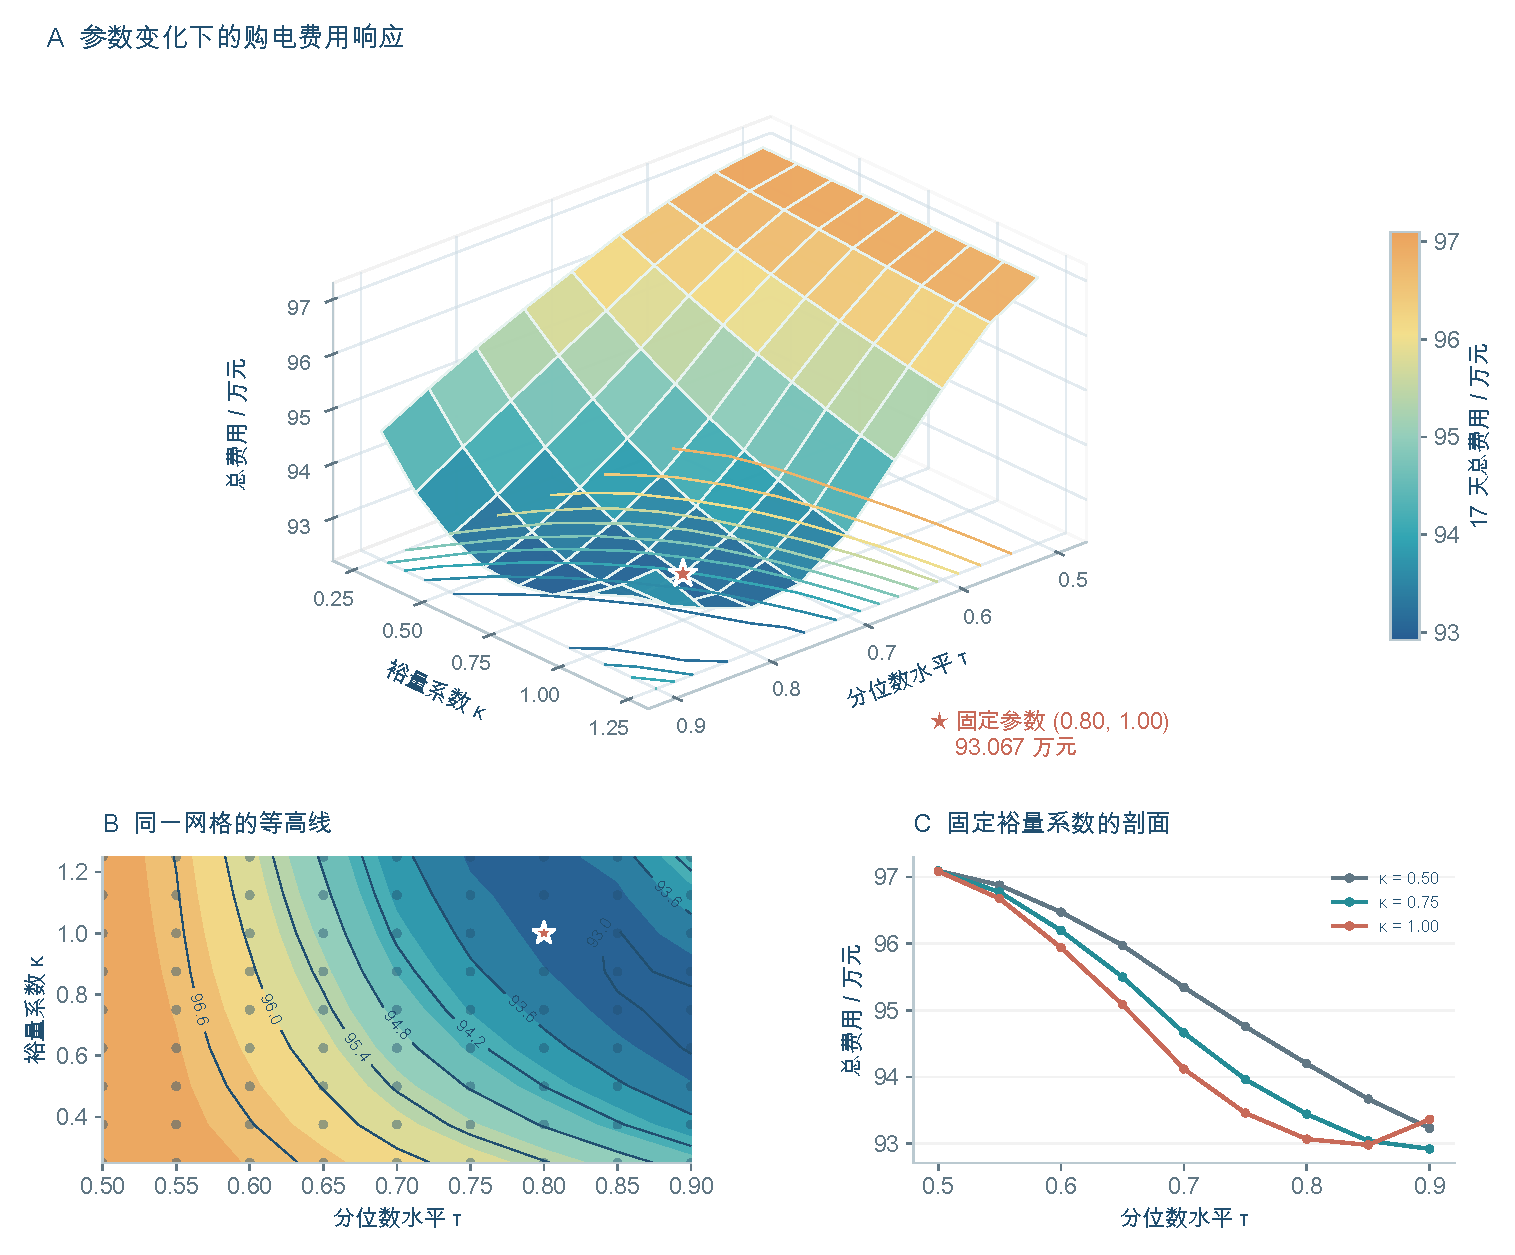
\includegraphics[width=\linewidth]{parameter_response.pdf}
\caption{一月15--31日的参数—费用响应面与敏感性剖面。A为81个实算节点连接形成的三维曲面及底面等高线，B为同一网格的俯视投影，C比较三组固定$\kappa$的费用变化；星号为所用参数$(0.8,1.0)$。节点间连接仅用于显示。}

\label{fig:resp}\end{figure}

为观察该选型对参数扰动的敏感程度，在同一严格执行器和同一因果残差历史下把候选网格加密为$\tau\in[0.50,0.90]$步长0.05、$\kappa\in[0.25,1.25]$步长0.125的81个组合，对一月15日至31日重放，共1377次日回放，效率、终端条件、价格与选型时一致。图\ref{fig:resp}显示费用沿两个方向的变化并不对称：提高分位数水平$\tau$带来的下降较明显，改变裕量系数$\kappa$较平缓，二者在相当范围内可以互相补偿，等高线因此呈现一条低费用带而不是孤立极小点。原参数$(0.8,1.0)$的一月费用为930672.15元，加密网格最低点$(0.9,0.75)$为929199.21元，相差1472.94元。

该差值只是一月开发期的描述性敏感性。本文没有据此对二月至十二月重新选型，也不能把1472.94元理解为全年可节省的金额；网格加密同样不证明连续参数空间中的全局最优。主方案参数保持$\tau=0.8$、$\kappa=1$不变。低费用带说明部分参数组合具有相近的开发期费用，支持在该邻域内讨论局部稳定性。


\subsection{二乘二消融及费用分解}
B0和B1分别采用基础预测配合基线执行器与小时MPC；B2和B3在对应执行器上加入安全裕量。表\ref{tab:q2}中所有年度数字覆盖相同334天。
\begin{table}[H]\centering\caption{第二问费用比较；Oracle仅为事后信息对照}\label{tab:q2}\small\begin{tabular}{lrrr}
\toprule
方案 & 计划费/元 & 紧急费/元 & 总费/元 \\
\midrule
B0 & 12,258,250.77 & 4,323,292.77 & 16,581,543.53 \\
B1 & 12,258,250.77 & 4,292,554.51 & 16,550,805.27 \\
B2 & 13,706,009.44 & 1,431,977.61 & 15,137,987.06 \\
B3 & 13,706,009.44 & 1,434,937.88 & 15,140,947.32 \\
fixedG\_oracle & 12,258,250.77 & 1,958,975.02 & 14,217,225.79 \\
full\_oracle & 12,245,046.92 & 0.00 & 12,245,046.92 \\
\bottomrule
\end{tabular}
\end{table}
\fig{margin_mechanism}{1}{安全裕量的证据链：一月分时残差、实际参数组合费用、因果历史裕量和费用瀑布图。山脊图仅描述一月8至31日残差，各组峰高分别归一化；红线为该描述样本的80\%分位，不是每天实际使用的固定裕量。参数热力图仅展示已运行组合，没有插值。}
B2相对B0节省1443556.47元，降幅8.7058\%。其正常计划费增加1447758.68元，但应急费减少2891315.15元，净效果为总费下降。应急电量为380769.33 kWh，无收益富余为3505784.13 kWh，高于B0约211万kWh的富余。安全裕量以更多承诺购电及富余换取昂贵缺口的减少，因此应以总费而非单独的应急费判断成败。

逐日成对比较中，B2有291日总费低于B0，43日更高；月内分布仍有负收益尾部，不能把全年降低解释为每一天均改善。

B1仅比B0低30738.26元，B3反而比B2高2960.27元。在冻结预测和既定结算机制下，重新求解并不必然增加有价值的信息，MPC还可能选择另一组预测最优、实际费用不同的动作。因此本文以B2为第二问主方案。
\fig{strategy_stability}{1}{第二问的逐日成对比较、月内节省分布、累计节省和应急费用尾部。小提琴图的横线为中位数；经验超越概率包含全部334天。收益分布用于稳定性诊断，不作独立样本显著性检验。}

\subsection{完美信息基准}
固定合同Oracle保持B0的$G$不变，仅允许储能提前知道整日实际路径；全信息Oracle还允许据实际路径选择日前$G$。两者保持相同效率、功率、SOC和日终条件。其费用分别为14217225.79和12245046.92元。B0与固定合同Oracle相差2364317.74元，提示固定承诺下存在调度信息空间；但该差额不保证能由因果算法实现。B2与全信息Oracle仍相差2892940.14元，不能据此声称尚有同等金额的可实现优化。


\subsection{全年储能运行规律}
把B2在334天中的实际控制轨迹按月聚合，可以观察安全裕量策略在全年的储能使用节律。图\ref{fig:soc3d}以物理时刻为横轴、月份为纵轴、月内逐时点日均储电量为高度，共11$\times$145个统计节点。各月形态一致：凌晨低价时段充至高位，日出后随光伏抬升先行放电，午后重新蓄电，晚峰再次放电，日初与日末都回到6 MWh。夏季月份的午间低谷更深、持续更久，与光伏电量高、净负荷小的季节结构相符。

曲面按月内各日等权平均，描述季节性运行特征；月份间连接仅用于显示，月均状态不能替代逐日轨迹的可行性检验。
\begin{figure}[H]\centering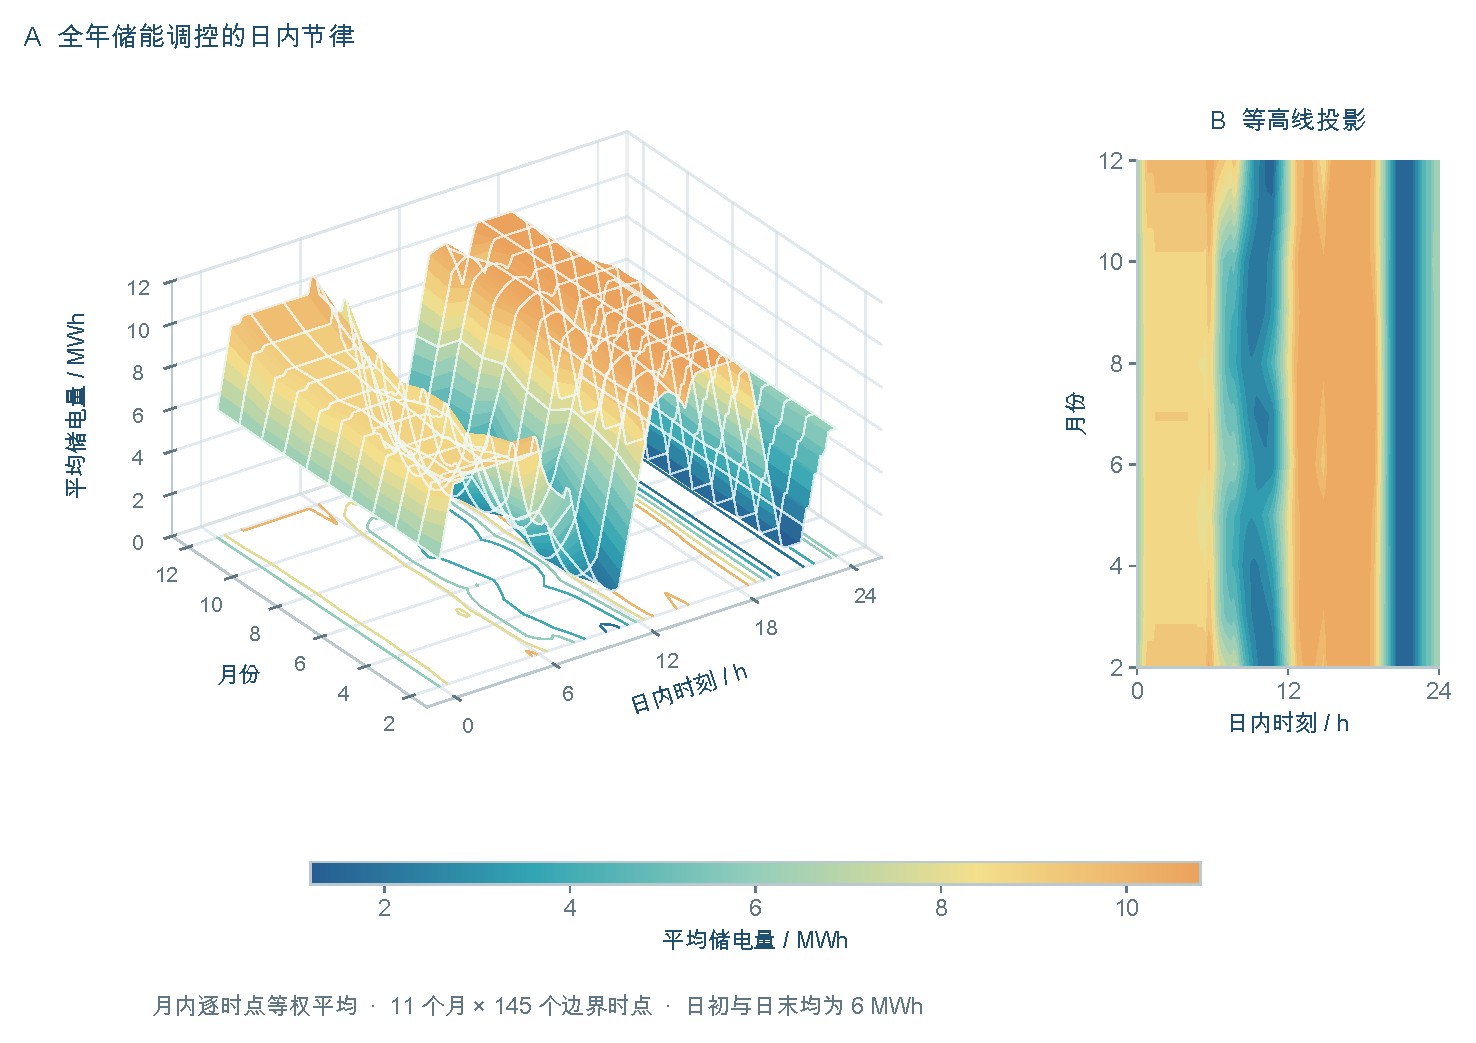
\includegraphics[width=\linewidth]{monthly_storage.pdf}
\caption{安全裕量策略的月均储电量曲面。A为日内时刻、月份与平均储电量的三维关系，B为同一数据的等高线投影。数据覆盖2025年2--12月，共$11\times145$个统计节点。}

\label{fig:soc3d}\end{figure}

\FloatBarrier
\section{第三问：合同更新及价值门控}
\subsection{预报积分与逐次合同结算}
每次发布的未来24小时光伏预报按发布时间索引，仅在发布后使用。对整点功率作分段线性插值并积分到10分钟电量，落在\ref{sec:time}节同一套槽网格上，使计划与结算共用一条时间轴；从发布时刻到首个整点的缺失起点采用第一条预报保持的边界近似。后续发布仅截取当天剩余区间，不能改写已执行槽。

设一次更新前后合同为$G^{old},G^{new}$，定义$\Delta G^+=[G^{new}-G^{old}]_+$、$\Delta G^-=[G^{old}-G^{new}]_+$。采用“原合同退款后收50\%违约费”的计费假设，增量费用为
\begin{equation}
J^{adj}_k=\sum_{t\ge k}p_t(1.5\Delta G_t^+-0.5\Delta G_t^-),\qquad
J_3=\sum_t p_tG_t^{0}+\sum_kJ^{adj}_k+\sum_t5p_tU_t.
\end{equation}
每次均相对当前合同计算，不能反复相对零点合同收取费用。若题意采用取消部分不退款、另收违约费，则应另作敏感性，不可与上述费用混用。

\subsection{固定更新的实测结果}
对无裕量和有裕量各比较零点固定、旧PV重规划和新PV重规划。旧PV组在严格控制下没有实质合同调整，其总费仅与零点组存在数值舍入差。新PV组则包含实际合同变化。
\begin{table}[H]\centering\caption{第三问334天费用分解（万元）；旧PV组与对应固定组数值相同，正文不重复列示}\small\begin{tabular}{lrrrr}
\toprule
方案 & 计划费/万元 & 调整费/万元 & 紧急费/万元 & 总费/万元 \\
\midrule
基线固定 & 1231.6402 & 0.0000 & 408.6698 & 1640.3101 \\
基线更新 & 1231.6402 & 40.1133 & 383.0000 & 1654.7535 \\
裕量固定 & 1378.3454 & 0.0000 & 134.6222 & 1512.9676 \\
裕量更新 & 1378.3454 & 43.7750 & 146.2228 & 1568.3432 \\
裕量门控 & 1378.3454 & 22.0776 & 111.8091 & 1512.2321 \\
\bottomrule
\end{tabular}
\end{table}

裕量零点固定费用15129676.16元，低于无裕量固定组1273424.41元。对裕量方案，每次使用新PV并重规划反而增加553755.87元。因而不能以“预报更新更频繁”直接推出费用下降。因此，合同更新的判断应同时考虑预测缺口与违约费用。图\ref{fig:rolling}展示了新预报重规划对照在一个指定日的决策过程。

\begin{figure}[H]\centering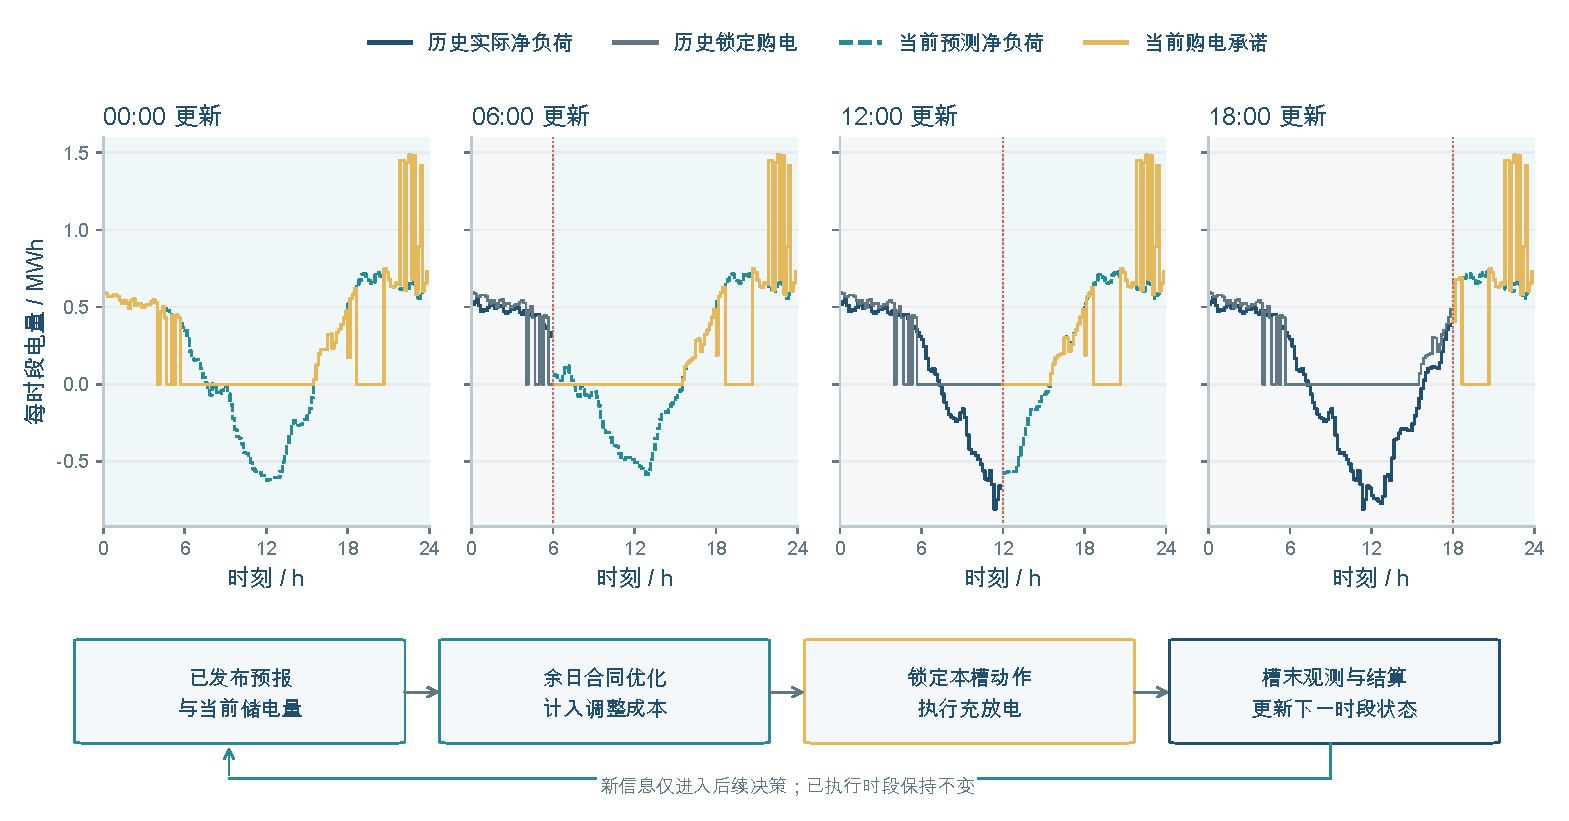
\includegraphics[width=\linewidth]{rolling_contract.pdf}
\caption{6月21日新预报重规划对照的四个决策快照。深色区域为已执行区间，浅色区域为待决策区间；各快照仅展示当时可用的预测及此前实际观测。该图用于解释更新机制，主方案仍为裕量零点固定。}\label{fig:rolling}
\end{figure}

\subsection{预期净收益门控}
在6、12、18点比较保持当前合同和接受新合同两种策略。以此前28日中最近20个可用完整历史日构造负荷及PV的联合残差路径，保留同日变量相关性和日内时序。历史PV残差对应同一发布时间的预报；不逐时段独立抽样。场景数不足7个历史日时回退为不更新。

每条场景分别计算两候选策略在余日的应急费用；预演中合同保持固定到日末，不假定未来还会得到何种新预报。两候选使用共同场景降低比较噪声。令
\begin{equation}
\widehat V_{keep}=\frac1S\sum_s J^{emg}_{keep,s},\quad
\widehat V_{update}=J^{adj}_k+\frac1S\sum_sJ^{emg}_{update,s}.
\end{equation}
仅当$\widehat V_{keep}-\widehat V_{update}>\theta$时更新；过去费用为沉没项，调整费只计一次。实际运行到下次发布时再重新评估。阈值在一月15日至31日从禁用、0、100、500及1000元中选择，最终为500元。

接受更新按6、12、18点分别为83、97和3次。这个差异描述本策略在当前数据及计费解释下的选择，不足以断言18点预报普遍无价值。

门控接受183次更新，共评估1002次，总费用15122320.83元。其应急费降至1118091.02元，但增加220775.53元调整费，相对裕量固定净节省仅7355.33元，约0.0486\%。全年7个月改善、4个月变差，见图\ref{fig:gate}。综合净节省幅度、月度稳定性与决策复杂度，本文保留裕量固定为简洁方案；门控在本组对照中总费用更低，但收益有限。事后收益只用于解释，不参与当时决策。
\begin{figure}[H]\centering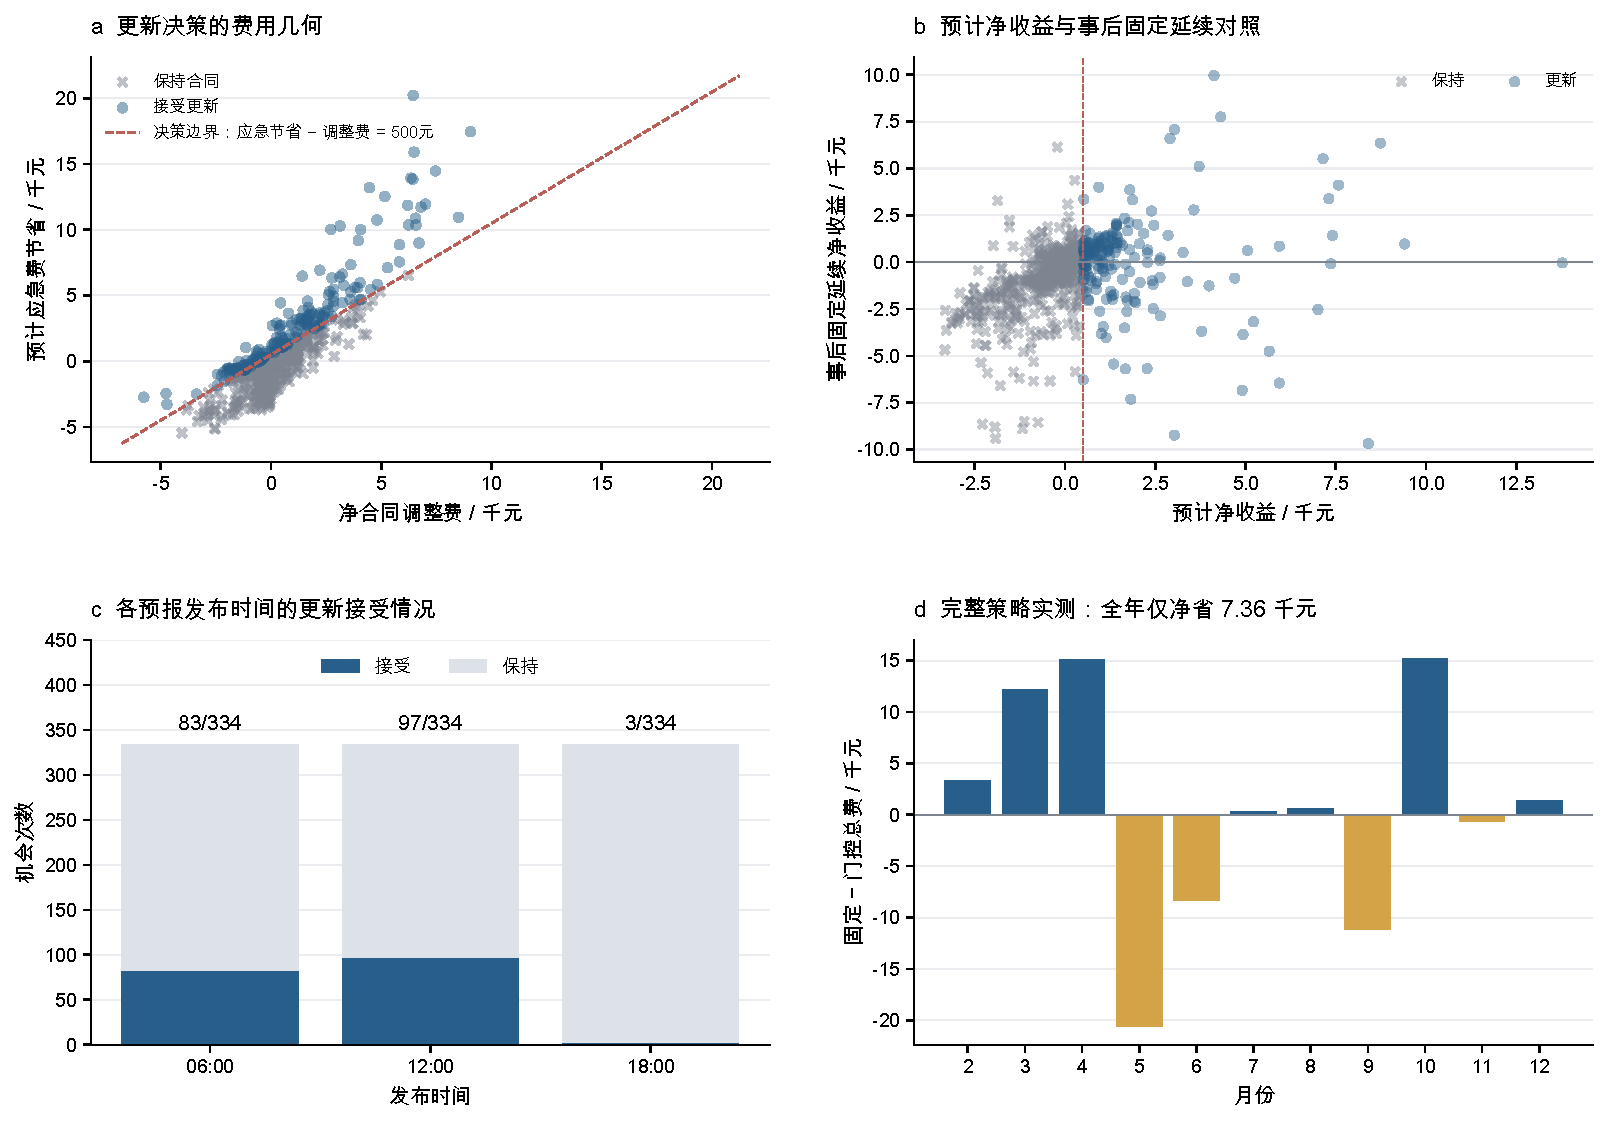
\includegraphics[width=\linewidth]{gate_decisions.pdf}\caption{第三问门控决策与回放检验。a中的净调整费可以为负；b是每次决策之后固定合同延续至日末的事后反事实，多个预演时域重叠，不能将其收益相加。d为完整运行策略的真实月度总费差，负值表示门控增费。}\label{fig:gate}\end{figure}

\FloatBarrier
\section{第四问：动态电价下的严格迁移}
\subsection{动态电价模型}
以$p_{d,t}$替换固定价格$p_t$，物理约束保持不变。日前策略最小化预测计划购电费，实际应急按$5p_{d,t}$结算，日内调整按$1.5p_{d,t}\Delta G^+-0.5p_{d,t}\Delta G^-$记账。价格同时进入计划、重规划与实际账本；仅对第二、三问已有动作重新计价不构成重优化。

本节的迁移\textbf{唯一改动是价格输入}：执行器、结算规则、效率、终端条件与第二、三问完全相同，安全裕量直接沿用一月冻结的$\tau=0.8$、$\kappa=1$，不在动态电价上重新选参。一月在动态电价下用B0重放作为热身，二月一日初始储电量为6000 kWh，评价区间仍为334天。价格可知性沿用“目标日整条曲线在零点可知”的条件假设，其影响在\ref{sec:price}节单独量化。

\subsection{对应第二问的结果}
\begin{table}[H]\centering\caption{第四问对应第二问的334天费用}\label{tab:q42}\small\begin{tabular}{lrrrr}
\toprule
方案 & 计划费/元 & 应急费/元 & 总费/元 & 应急电量/kWh \\
\midrule
B0 无裕量 & 12,804,733.57 & 4,510,680.10 & 17,315,413.67 & 1,110,891 \\
B2 安全裕量 & 14,318,165.75 & 1,510,856.77 & 15,829,022.52 & 380,769 \\
\bottomrule
\end{tabular}
\end{table}
安全裕量节省1486391.15元，降幅8.5842\%；固定电价下同一策略的降幅是8.7058\%。计划费增加约151万元、应急费减少约300万元的机制原样成立。在本题动态电价样本中，安全裕量仍能降低总购电费用。

\subsection{对应第三问的结果}
\begin{table}[H]\centering\caption{第四问对应第三问的334天费用分解（万元）}\label{tab:q43}\small\begin{tabular}{lrrrr}
\toprule
方案 & 计划费/万元 & 调整费/万元 & 应急费/万元 & 总费/万元 \\
\midrule
基线零点固定 & 1287.9892 & 0.0000 & 427.1681 & 1715.1574 \\
基线旧PV更新 & 1287.9892 & 0.0000 & 427.1681 & 1715.1574 \\
基线新PV更新 & 1287.9892 & 42.8684 & 392.8964 & 1723.7540 \\
裕量零点固定 & 1440.8445 & 0.0000 & 141.4456 & 1582.2900 \\
裕量旧PV更新 & 1440.8445 & 0.0000 & 141.4456 & 1582.2900 \\
裕量新PV更新 & 1440.8445 & 46.6572 & 147.8673 & 1635.3690 \\
\bottomrule
\end{tabular}
\end{table}
旧PV组与零点组仅差浮点舍入，与固定电价时同样没有实质合同调整。新PV重规划在动态电价下依然\textbf{更贵}，增加530789.48元（3.3546\%）；固定电价下为553755.87元（3.6601\%）。第三问“获得新预报不必然值得支付调整代价”的结论因此不随电价形式改变。

\begin{table}[H]\centering\caption{同一策略在两种电价下的总费对照}\label{tab:q4cmp}\small\begin{tabular}{lrrr}
\toprule
方案 & 固定电价/元 & 动态电价/元 & 差额/元 \\
\midrule
Q2 基线 B0 & 16,581,543.53 & 17,315,413.67 & +733,870.14 \\
Q2 裕量 B2 & 15,137,987.06 & 15,829,022.52 & +691,035.46 \\
Q3 基线零点固定 & 16,403,100.57 & 17,151,573.70 & +748,473.13 \\
Q3 裕量零点固定 & 15,129,676.16 & 15,822,900.47 & +693,224.31 \\
Q3 裕量新PV更新 & 15,683,432.03 & 16,353,689.95 & +670,257.92 \\
\bottomrule
\end{tabular}
\end{table}
各方案在动态电价下的总费增加约67万至75万元，反映价格输入与调度共同变化后的净结果；所比较方案的相对排序一致。图\ref{fig:pricecmp}进一步展示费用构成及月度节省。
\begin{figure}[H]\centering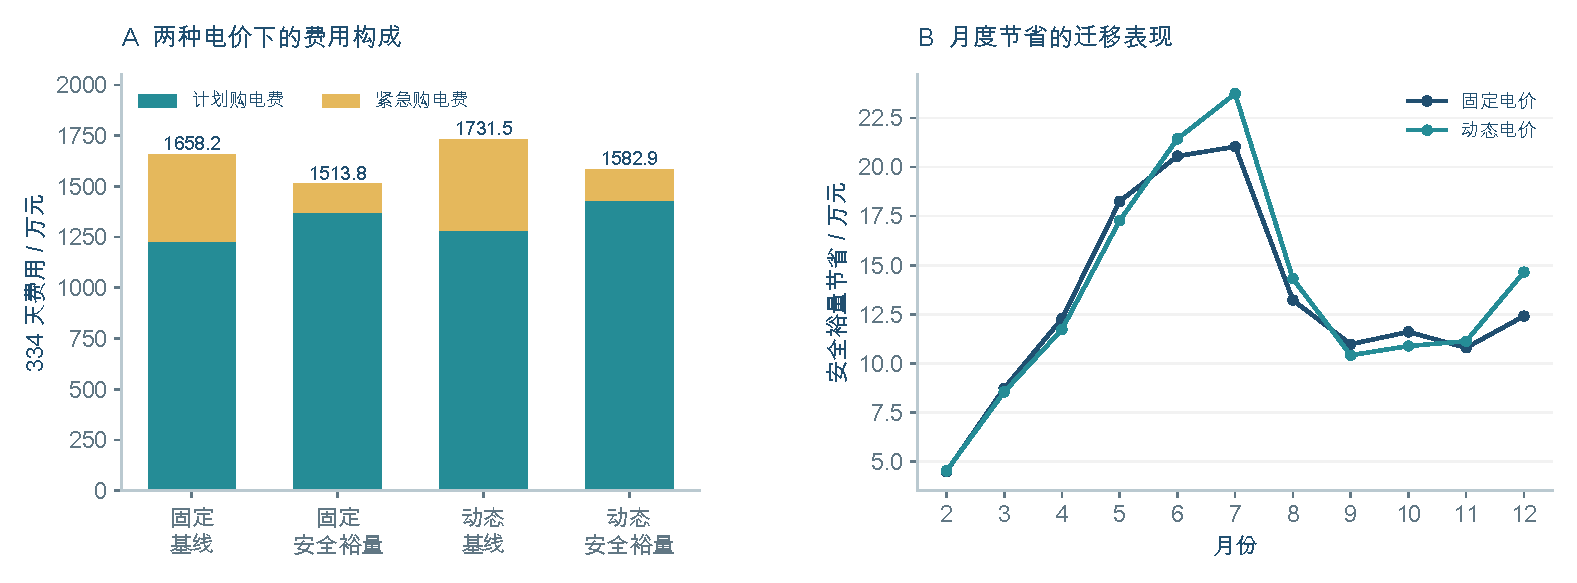
\includegraphics[width=\linewidth]{dynamic_price_comparison.pdf}
\caption{固定与动态电价下的安全裕量效果。A比较334天的计划费与紧急费，B展示各月相对无裕量基线的净节省。}\label{fig:pricecmp}\end{figure}

\subsection{固定计划执行下的残差机制}
在本组固定承诺实验中，对334天逐时段比较固定与动态电价下的B2，紧急电量$U_t$、富余电量$W_t$与$C_t-G_t-D_t$的最大差均约为$2.2\times10^{-8}$ kWh，而充电量$C_t$的最大差为833.333 kWh。这表明电价可显著改变储能动作，却未改变该执行规则下的实际缺口。

记日前规划使用的负荷与光伏为$L_t^p,V_t^p$，基线使用原始预测，安全裕量策略使用修正预测。当日前计划富余为零且执行计划充放电动作时，有
\[
G_t=L_t^p+C_t^p-V_t^p-D_t^p,\qquad C_t=C_t^p,\quad D_t=D_t^p.
\]
代入能量平衡可得
\begin{equation}\label{eq:inv}
U_t=[(L_t-L_t^p)-(V_t-V_t^p)]_+,\qquad
W_t=[(V_t-V_t^p)-(L_t-L_t^p)]_+.
\end{equation}
因此，在这些条件下，应急与富余由净负荷残差决定，电价只通过调度与合同量改变购电的时段分配。安全裕量改变的是残差分布，因而可在保持参数不变时迁移到动态电价。该性质依赖于无计划富余与既定动作执行，不能推广为所有储能控制器均与电价无关。

\subsection{价格信息的经济价值}\label{sec:price}
设置对照组：按固定代表日电价制定计划，按真实动态电价结算。其总费15967316.98元，比真正使用动态曲线的15829022.52元高138294.46元，即0.8661\%。两者应急电量同为380769.33 kWh，印证上节结论：这0.87\%完全来自计划购电在时间上的重新分配，与应急无关。

上述0.8661\%是本年度数据和指定固定价格基线下的实测费用差，并非价格未知时损失的普遍上界。若目标日电价不能提前获得，需要将价格预测纳入日前信息集，并重新评价策略。

\FloatBarrier
\section{模型检验与讨论}
\subsection{可行性及信息时序检验}
对调度轨迹逐时段复算能量平衡、储电量递推、功率与容量边界、初末状态及总费用。第二问B2的最大物理残差为$4.55\times10^{-13}$ kWh，小于$10^{-6}$ kWh容差。第四问的8组对照覆盖2672个运行日、384768个时段，均满足上述约束。

为检验决策是否依赖尚未获得的信息，将目标日实际序列替换为零值后重新生成动作，既定储能指令与合同修订保持一致；实际序列仅影响后续结算。第三问同时检查预报发布时间、已执行合同保持不变和调整费用逐次累计，以保证比较使用相同的信息边界。

\subsection{敏感性与适用范围}
代表日积分方式的费用跨度为0.68\%。若将90\%解释为往返效率，优化费用由35126.95元变为33801.50元。两者分别反映离散方式与效率假设的影响。安全裕量在所考察的一月参数网格内呈现低费用带，但不能据此推断所有参数或其他年份均有同样表现。

本文采用每日初末储电量6000 kWh、母线侧功率限制以及减购退款后收取50\%违约费的假设。跨日储能、其他计费方式与价格预测误差均可能改变费用结构。历史分位数与联合残差场景依赖误差的可迁移性，极端天气和负荷突变仍可能导致较高应急费用。10分钟电量模型适用于能量管理层，不能直接描述秒级功率控制。动态电价实验沿用裕量参数，未将第三问门控阈值的效果外推至第四问。

\FloatBarrier
\section{结论}
本文建立统一的微网储能与购电调控模型，将预测、计划、执行和结算置于明确的信息时序下。代表日优化相对无储能降低费用26.90\%；历史净负荷残差安全裕量在334天回放中降低费用8.71\%，其经济机制是以更多计划购电抵消高价应急缺口。

合同更新实验表明，新预报的价值应由扣除调整成本后的净收益衡量。逐次更新可能增费，预期净收益门控相对裕量固定策略仅节省0.0486\%，说明更频繁的优化不必然具有足够的经济价值。动态电价下，裕量策略仍降费8.58\%，新预报重规划仍增费3.35\%，支持在本题价格样本中保留相同的策略选择。

参数费用曲面揭示了开发期的低费用区域，储电量曲面呈现相近的日内充放节律。固定计划执行下的残差恒等式进一步解释了裕量跨电价场景迁移的原因。模型的实用价值在于以可实现的信息和完整费用为依据选择调度策略，并将模型假设、物理可行性与经济收益分别检验。

\begin{thebibliography}{9}
\bibitem{problem} 全国大学生数学建模竞赛组委会. 2026年高教社杯全国大学生数学建模竞赛C题：微网与外部电网电力调控策略及附件1--5[Z]. 2026.
\bibitem{parisio} Parisio A, Rikos E, Glielmo L. A model predictive control approach to microgrid operation optimization[J]. IEEE Transactions on Control Systems Technology, 2014, 22(5): 1813--1827. DOI: \href{https://doi.org/10.1109/TCST.2013.2295737}{10.1109/TCST.2013.2295737}.
\bibitem{boyd} Boyd S, Vandenberghe L. Convex Optimization[M]. Cambridge: Cambridge University Press, 2004. \url{https://web.stanford.edu/~boyd/cvxbook/}.
\end{thebibliography}
\clearpage

\appendix\small
\FloatBarrier
\section{第二问四个指定日调度明细}
采用安全裕量策略B2。费用为计划费与紧急费之和，连续紧急时段按相邻区间合并，判断阈值为$10^{-6}$ kWh。时段采用第\ref{sec:time}节的物理区间。
\Needspace{15\baselineskip}
\subsubsection*{2025-03-20}

\begin{center}\small\begin{tabular}{lr}
\toprule
时段 & 购电量/kWh \\
\midrule
10:00--10:10 & 0.000 \\
12:00--12:10 & 538.078 \\
14:00--14:10 & 0.000 \\
16:00--16:10 & 449.121 \\
18:00--18:10 & 717.524 \\
20:00--20:10 & 0.000 \\
\bottomrule
\end{tabular}
\quad\begin{tabular}{lrr}
\toprule
时段 & 充电量/kWh & 放电量/kWh \\
\midrule
00:00--04:00 & 4500.000 & 0.000 \\
04:00--08:00 & 833.333 & 4820.169 \\
08:00--12:00 & 6062.807 & 3819.831 \\
12:00--16:00 & 5278.798 & 546.700 \\
16:00--20:00 & 0.000 & 5655.091 \\
20:00--24:00 & 5333.333 & 2984.908 \\
\bottomrule
\end{tabular}
\end{center}
全天计划购电量 69403.586 kWh，总费用 47,213.32 元，其中紧急费 4,830.84 元；日初、日末储电量均为6000 kWh。
\begin{center}\small
\begin{tabular}{lrlr}\toprule
紧急购电时段 & 电量/kWh & 紧急购电时段 & 电量/kWh\\\midrule
00:20--00:30 & 10.820 \ & 12:20--13:40 & 565.833 \ \\
01:00--01:40 & 113.352 \ & 15:30--17:00 & 404.069 \ \\
03:10--03:30 & 45.273 \ & 17:20--17:30 & 6.655 \ \\
03:40--04:00 & 10.987 \ & 18:40--19:00 & 30.131 \ \\
09:50--10:00 & 16.348 \ & 21:10--21:40 & 9.856 \ \\
11:00--11:40 & 267.483 \ & 23:30--23:50 & 3.640 \ \\
\bottomrule\end{tabular}\end{center}

\Needspace{15\baselineskip}
\subsubsection*{2025-06-21}

\begin{center}\small\begin{tabular}{lr}
\toprule
时段 & 购电量/kWh \\
\midrule
10:00--10:10 & 0.000 \\
12:00--12:10 & 0.000 \\
14:00--14:10 & 0.000 \\
16:00--16:10 & 195.842 \\
18:00--18:10 & 220.356 \\
20:00--20:10 & 0.000 \\
\bottomrule
\end{tabular}
\quad\begin{tabular}{lrr}
\toprule
时段 & 充电量/kWh & 放电量/kWh \\
\midrule
00:00--04:00 & 0.000 & 0.000 \\
04:00--08:00 & 418.971 & 4320.000 \\
08:00--12:00 & 6904.691 & 0.000 \\
12:00--16:00 & 3343.004 & 0.000 \\
16:00--20:00 & 0.000 & 5781.027 \\
20:00--24:00 & 5333.333 & 2858.973 \\
\bottomrule
\end{tabular}
\end{center}
全天计划购电量 39985.338 kWh，总费用 24,257.70 元，其中紧急费 527.25 元；日初、日末储电量均为6000 kWh。
\begin{center}\small
\begin{tabular}{lrlr}\toprule
紧急购电时段 & 电量/kWh & 紧急购电时段 & 电量/kWh\\\midrule
01:20--01:30 & 4.811 \ & 05:50--06:20 & 24.340 \ \\
01:50--02:00 & 5.781 \ & 07:10--07:50 & 95.962 \ \\
04:00--04:10 & 1.894 \ & 09:00--09:10 & 5.668 \ \\
\bottomrule\end{tabular}\end{center}

\Needspace{15\baselineskip}
\subsubsection*{2025-09-23}

\begin{center}\small\begin{tabular}{lr}
\toprule
时段 & 购电量/kWh \\
\midrule
10:00--10:10 & 0.000 \\
12:00--12:10 & 495.788 \\
14:00--14:10 & 0.000 \\
16:00--16:10 & 571.697 \\
18:00--18:10 & 787.811 \\
20:00--20:10 & 0.000 \\
\bottomrule
\end{tabular}
\quad\begin{tabular}{lrr}
\toprule
时段 & 充电量/kWh & 放电量/kWh \\
\midrule
00:00--04:00 & 4500.000 & 0.000 \\
04:00--08:00 & 833.333 & 6014.927 \\
08:00--12:00 & 5873.974 & 2625.073 \\
12:00--16:00 & 5114.639 & 260.776 \\
16:00--20:00 & 0.000 & 5784.185 \\
20:00--24:00 & 5333.333 & 2855.815 \\
\bottomrule
\end{tabular}
\end{center}
全天计划购电量 71761.883 kWh，总费用 48,209.42 元，其中紧急费 3,641.20 元；日初、日末储电量均为6000 kWh。
\begin{center}\small
\begin{tabular}{lrlr}\toprule
紧急购电时段 & 电量/kWh & 紧急购电时段 & 电量/kWh\\\midrule
00:40--00:50 & 18.879 \ & 16:00--16:10 & 17.736 \ \\
02:00--02:20 & 23.198 \ & 16:20--16:40 & 6.349 \ \\
05:00--05:10 & 11.088 \ & 18:10--18:30 & 33.963 \ \\
06:50--07:10 & 19.695 \ & 20:00--20:30 & 78.072 \ \\
07:50--08:00 & 3.058 \ & 20:50--21:10 & 54.838 \ \\
09:30--10:20 & 200.726 \ & 21:20--21:30 & 30.480 \ \\
10:40--11:00 & 10.011 \ & 22:20--22:30 & 14.773 \ \\
14:10--15:10 & 268.848 \ &  &  \\
\bottomrule\end{tabular}\end{center}

\Needspace{15\baselineskip}
\subsubsection*{2025-12-21}

\begin{center}\small\begin{tabular}{lr}
\toprule
时段 & 购电量/kWh \\
\midrule
10:00--10:10 & 0.000 \\
12:00--12:10 & 958.629 \\
14:00--14:10 & 0.000 \\
16:00--16:10 & 805.047 \\
18:00--18:10 & 744.862 \\
20:00--20:10 & 0.000 \\
\bottomrule
\end{tabular}
\quad\begin{tabular}{lrr}
\toprule
时段 & 充电量/kWh & 放电量/kWh \\
\midrule
00:00--04:00 & 4500.000 & 0.000 \\
04:00--08:00 & 1666.667 & 1508.333 \\
08:00--12:00 & 5833.333 & 7806.667 \\
12:00--16:00 & 8333.333 & 2835.000 \\
16:00--20:00 & 0.000 & 5614.064 \\
20:00--24:00 & 5333.333 & 3025.936 \\
\bottomrule
\end{tabular}
\end{center}
全天计划购电量 101100.136 kWh，总费用 67,816.35 元，其中紧急费 2,416.92 元；日初、日末储电量均为6000 kWh。
\begin{center}\small
\begin{tabular}{lrlr}\toprule
紧急购电时段 & 电量/kWh & 紧急购电时段 & 电量/kWh\\\midrule
03:00--03:10 & 13.363 \ & 18:20--19:00 & 54.040 \ \\
03:30--03:50 & 77.487 \ & 19:50--20:00 & 11.160 \ \\
10:20--11:30 & 564.551 \ & 22:50--23:00 & 1.635 \ \\
12:40--12:50 & 9.139 \ & 23:30--23:40 & 7.990 \ \\
\bottomrule\end{tabular}\end{center}

\clearpage
\FloatBarrier
\section{第三问四个指定日调度明细}
采用裕量零点固定策略，调整后的购电计划与原承诺相同，合同调整费为零。费用包括计划费与紧急费；指定时段购电、分段充放电及紧急购电明细如下。
\Needspace{15\baselineskip}
\subsubsection*{2025-03-20}

\begin{center}\small\begin{tabular}{lr}
\toprule
时段 & 购电量/kWh \\
\midrule
10:00--10:10 & 0.000 \\
12:00--12:10 & 599.713 \\
14:00--14:10 & 0.000 \\
16:00--16:10 & 642.201 \\
18:00--18:10 & 717.524 \\
20:00--20:10 & 0.000 \\
\bottomrule
\end{tabular}
\quad\begin{tabular}{lrr}
\toprule
时段 & 充电量/kWh & 放电量/kWh \\
\midrule
00:00--04:00 & 4500.000 & 0.000 \\
04:00--08:00 & 833.333 & 5840.742 \\
08:00--12:00 & 6550.887 & 2799.258 \\
12:00--16:00 & 5945.791 & 1482.309 \\
16:00--20:00 & 0.000 & 5655.091 \\
20:00--24:00 & 5333.333 & 2984.908 \\
\bottomrule
\end{tabular}
\end{center}
全天计划购电量 73185.747 kWh，总费用 48,347.77 元，其中紧急费 3,565.06 元；日初、日末储电量均为6000 kWh。
\begin{center}\small
\begin{tabular}{lrlr}\toprule
紧急购电时段 & 电量/kWh & 紧急购电时段 & 电量/kWh\\\midrule
00:20--00:30 & 10.820 \ & 09:40--11:40 & 704.563 \ \\
01:00--01:40 & 113.352 \ & 17:20--17:30 & 15.544 \ \\
03:10--03:30 & 45.273 \ & 18:40--19:00 & 30.061 \ \\
03:40--04:00 & 10.987 \ & 21:10--21:40 & 9.856 \ \\
08:10--08:30 & 57.907 \ & 23:30--23:50 & 3.640 \ \\
09:00--09:10 & 3.489 \ &  &  \\
\bottomrule\end{tabular}\end{center}

\Needspace{15\baselineskip}
\subsubsection*{2025-06-21}

\begin{center}\small\begin{tabular}{lr}
\toprule
时段 & 购电量/kWh \\
\midrule
10:00--10:10 & 0.000 \\
12:00--12:10 & 0.000 \\
14:00--14:10 & 0.000 \\
16:00--16:10 & 224.337 \\
18:00--18:10 & 171.822 \\
20:00--20:10 & 0.000 \\
\bottomrule
\end{tabular}
\quad\begin{tabular}{lrr}
\toprule
时段 & 充电量/kWh & 放电量/kWh \\
\midrule
00:00--04:00 & 0.000 & 0.000 \\
04:00--08:00 & 97.885 & 4320.000 \\
08:00--12:00 & 7291.479 & 1.385 \\
12:00--16:00 & 3279.012 & 0.000 \\
16:00--20:00 & 0.000 & 5781.024 \\
20:00--24:00 & 5333.333 & 2858.976 \\
\bottomrule
\end{tabular}
\end{center}
全天计划购电量 39989.708 kWh，总费用 23,415.96 元，其中紧急费 27.02 元；日初、日末储电量均为6000 kWh。
\begin{center}\small
\begin{tabular}{lrlr}\toprule
紧急购电时段 & 电量/kWh & 紧急购电时段 & 电量/kWh\\\midrule
01:20--01:30 & 4.811 \ & 04:00--04:10 & 1.939 \ \\
01:50--02:00 & 5.781 \ &  &  \\
\bottomrule\end{tabular}\end{center}

\Needspace{15\baselineskip}
\subsubsection*{2025-09-23}

\begin{center}\small\begin{tabular}{lr}
\toprule
时段 & 购电量/kWh \\
\midrule
10:00--10:10 & 0.000 \\
12:00--12:10 & 438.775 \\
14:00--14:10 & 0.000 \\
16:00--16:10 & 595.756 \\
18:00--18:10 & 787.811 \\
20:00--20:10 & 0.000 \\
\bottomrule
\end{tabular}
\quad\begin{tabular}{lrr}
\toprule
时段 & 充电量/kWh & 放电量/kWh \\
\midrule
00:00--04:00 & 4500.000 & 0.000 \\
04:00--08:00 & 833.333 & 5058.319 \\
08:00--12:00 & 5833.333 & 3581.681 \\
12:00--16:00 & 5703.379 & 704.737 \\
16:00--20:00 & 0.000 & 5784.185 \\
20:00--24:00 & 5333.333 & 2855.815 \\
\bottomrule
\end{tabular}
\end{center}
全天计划购电量 75534.080 kWh，总费用 48,438.17 元，其中紧急费 1,276.88 元；日初、日末储电量均为6000 kWh。
\begin{center}\small
\begin{tabular}{lrlr}\toprule
紧急购电时段 & 电量/kWh & 紧急购电时段 & 电量/kWh\\\midrule
00:40--00:50 & 18.879 \ & 20:00--20:30 & 78.072 \ \\
02:00--02:20 & 23.198 \ & 20:50--21:10 & 54.838 \ \\
05:00--05:10 & 11.020 \ & 21:20--21:30 & 30.480 \ \\
17:30--17:40 & 0.579 \ & 22:20--22:30 & 14.773 \ \\
18:10--18:30 & 32.933 \ &  &  \\
\bottomrule\end{tabular}\end{center}

\Needspace{15\baselineskip}
\subsubsection*{2025-12-21}

\begin{center}\small\begin{tabular}{lr}
\toprule
时段 & 购电量/kWh \\
\midrule
10:00--10:10 & 0.000 \\
12:00--12:10 & 1018.506 \\
14:00--14:10 & 0.000 \\
16:00--16:10 & 810.495 \\
18:00--18:10 & 744.862 \\
20:00--20:10 & 0.000 \\
\bottomrule
\end{tabular}
\quad\begin{tabular}{lrr}
\toprule
时段 & 充电量/kWh & 放电量/kWh \\
\midrule
00:00--04:00 & 4500.000 & 0.000 \\
04:00--08:00 & 1666.667 & 1508.333 \\
08:00--12:00 & 5833.333 & 7806.667 \\
12:00--16:00 & 7948.901 & 2523.610 \\
16:00--20:00 & 0.000 & 5614.064 \\
20:00--24:00 & 5333.333 & 3025.936 \\
\bottomrule
\end{tabular}
\end{center}
全天计划购电量 101377.694 kWh，总费用 66,217.94 元，其中紧急费 875.79 元；日初、日末储电量均为6000 kWh。
\begin{center}\small
\begin{tabular}{lrlr}\toprule
紧急购电时段 & 电量/kWh & 紧急购电时段 & 电量/kWh\\\midrule
03:00--03:10 & 13.363 \ & 16:50--17:00 & 9.992 \ \\
03:30--03:50 & 77.487 \ & 18:20--19:00 & 54.039 \ \\
11:10--11:20 & 11.218 \ & 19:50--20:00 & 11.160 \ \\
12:40--13:10 & 19.223 \ & 22:50--23:00 & 1.635 \ \\
15:20--15:30 & 6.647 \ & 23:30--23:40 & 7.990 \ \\
16:20--16:30 & 13.682 \ &  &  \\
\bottomrule\end{tabular}\end{center}

\clearpage
\section{核心建模程序}
以下摘录对应正文的约束构造、预测修正与合同决策，使用 Python、NumPy 和 SciPy 实现。$G,C,D,U,W,E$分别对应购电、充电、放电、应急、富余和储电量；所有电量单位均为 kWh。完整函数及运行入口见随附源码。

\subsection{稀疏物理约束与充放电互斥}
将各时段变量依次拼接为向量，前两组等式分别表示能量平衡和储电量递推。二元变量仅在启用互斥约束时加入；若线性松弛存在同时充放电，则重新求解混合整数模型。
\lstinputlisting[firstline=99,lastline=139,caption={储能约束矩阵与变量边界}]{../../src/core/model.py}
\lstinputlisting[firstline=77,lastline=86,caption={物理校验与整数模型回退}]{../../src/core/solver.py}

\clearpage
\subsection{历史残差安全裕量与槽末结算}
残差库只接收目标日前已发布的整日数据；每个四小时桶内对原始净负荷残差求分位数。正文采用 $\tau=0.8$、$\kappa=1$，历史不足七日时保持零裕量。结算函数读取已经锁定的充放电动作，实际负荷与光伏仅用于计算应急和富余电量。
\lstinputlisting[firstline=36,lastline=64,caption={因果残差库与分时分位数裕量}]{../../src/q2/residual_margin.py}
\lstinputlisting[firstline=107,lastline=123,caption={锁定动作后的实际电量结算}]{../../src/q2/strict_execution.py}

\clearpage
\subsection{分段合同调整费与余日重规划}
主模型采用减购退款解释。相对当前合同，增购的增量费用为 $1.5p$，减购为 $-0.5p$；辅助变量满足 $a\ge G-G^{\mathrm{old}}$、$a\ge0$，将分段费用写成线性目标。函数仅接收尚未执行时段的向量，日终储电量保持6000 kWh。
\lstinputlisting[firstline=10,lastline=14,caption={合同增减量的实际计费}]{../../src/q3/planning.py}
\lstinputlisting[firstline=17,lastline=42,caption={含调整费用的线性规划及混合整数求解}]{../../src/q3/planning.py}
\lstinputlisting[firstline=45,lastline=58,caption={物理可行性与费用常数项核验}]{../../src/q3/planning.py}

\clearpage
\subsection{联合残差情景与更新收益门控}
对保持合同与更新合同使用同一组历史日残差路径，保留负荷和光伏误差的日内联合结构。两个候选均延续至当日结束，不预先假定之后门控的决定。收益为保持方案应急费减去更新方案应急费及调整费；仅当情景平均收益超过一月选定的500元阈值时接受更新。
\lstinputlisting[firstline=39,lastline=55,caption={最近28日内最多20条联合残差路径}]{../../src/q3/voi.py}
\lstinputlisting[firstline=66,lastline=79,caption={候选动作延续与情景应急费用}]{../../src/q3/voi.py}
\lstinputlisting[firstline=93,lastline=106,caption={新合同提案与预期净收益判定}]{../../src/q3/voi.py}

第四问沿用上述约束和执行过程，将价格向量替换为目标日动态电价。本文未将第三问的门控阈值直接用于第四问。


\end{document}
